\documentclass[10pt,a4paper]{article}
\usepackage[margin=1.5cm]{geometry}
\usepackage{graphicx}
\usepackage{multicol}
\usepackage{amsmath}
\usepackage{amssymb}
\usepackage{booktabs}
\usepackage{hyperref}

\twocolumn
\raggedright

\title{\textbf{Dynamic Pricing Model for Vande Bharat Express: Implementation and Revenue Analysis}}
\author{\begin{tabular}{c}
Gudaru Pragathi (25BM6JP10) \\ 
Sanket Wathore (25BM6JP44) \\ 
Srirang Nabar (25BM6JP53) \\ 
Boddu Harsha (25BM6JP08) \\ 
Konda Spandana (25BM6JP24) \\ 
Chetti Sai Srikar (25BM6JP09) \\
\textit{SCA Group 9 PGDBA}
\end{tabular}}
\date{}

\begin{document}

\maketitle

\begin{abstract}
This report implements the dynamic pricing strategy proposed by Singh et al. (2023) for Indian Railways on the Vande Bharat Express dataset. The model uses inter-temporal and demand-based pricing factors to adjust fares dynamically. Our analysis of 84 Vande Bharat trains demonstrates the potential for significant revenue optimization while maintaining fare affordability within the 0.8x to 1.4x base fare range.
\end{abstract}

\section{Overview, Data Generation and Variable Definitions}

\subsection{Background \& Context}

The Vande Bharat Express is India's semi-high-speed intercity train service. It was started by
Indian Railways in February 2019 and is made at the Integral Coach Factory in Chennai. As of
March 2026, it runs 164 daily services across 82 routes that cover all 16 railway zones and
274+ districts. The fleet has 8, 16, and 20-coach setups, and one sleeper variant on the
Howrah–Kamakhya route that started in January 2026. The dataset includes all 82 route pairs,
with 114 variables per row. It comes from the official IRCTC fare structure via vbooking.in,
schedule data from 24coaches.com that has been checked against IndiaRailInfo, and the route
list from the publicly available Indian Railways compilation called "Vande Bharat Express
Complete Train List, All 82 Routes Operational as of March 2026."

\subsection{Occupancy Simulation Methodology}

Live CNF data, which stands for Confirmed Seat Availability, is not in the public domain.
Therefore, based on a seeded deterministic mathematical model of 4 modules, the occupancy
for the next 20 days is estimated. The initial part defines the base demand, which lies in the
range between 40 and 75 percent on a per-route basis. It involves the use of the formula base
$= 40 + sin(train index \times 31 + direction \times 7) \times 35$. This ensures that popular routes like
Delhi–Varanasi automatically get a higher score than regional ones and reproducibility of
results is assured. The second one uses a ramp-up of bookings with ramp $= (20 - day)/20 \times 20$,
which is another 20p closer to the date of travel and reflects the actual booking concentration
of Indian Railways which is from 7 to 14 days prior to departure. Paste text generated by AI
tools like ChatGPT, Claude, or other AI systems. You can then detect if it appears AI-generated
or humanize it to make it sound more natural.A further 15 percentage point weekend premium
for Saturday and Sunday departures to tap higher leisure and pilgrimage demand. The equation
for how noise varies over the course of the day is given by noise $= (\sin(train index \times 100 + day
\times 17 + direction \times 13) - 0.5) \times 20$, which introduces a realistic, day-to-day variation of about
±10 percentage points. The values of all the four components will be summed, rounded and
clamped between 5 and 100. The Executive Chair Car occupancy will be 92\% of that for chair
car for the same route and day as it fills slower being a smaller premium class. The up and down
directions are independently seeded to maintain directional asymmetry. The two revenue
variables are as follows: assume the CC and EC revenue per run equals their respective fare
multiplied by seats multiplied by average occupancy divided 100. The Revenue Gap is defined
as the difference between maximum possible revenue at full occupancy and actual estimated
revenue. The Priority flag is HIGH if the gap is more than Rs. 15 lakh, MEDIUM if it is more
than Rs. 8 lakh and LOW otherwise.

\subsection{Key Assumptions and Limitations}

Prices are based on the General Quota published rates as of March 2026. They do not include
dynamic pricing, concession categories, or any changes made after the budget. The 1.30x
Tatkal multiplier is a planning tool, not the official schedule for that route. The seat capacity
for 16-coach trains is always the same: 780 CC seats and 104 EC seats. This means that 8-
coach and 20-coach trains have a capacity estimation error that can be fixed by looking at the
coach count in the dataset. The fare includes a catering fee of about Rs. 80-150 per passenger,
which is not broken down. The revenue numbers only show one way per run and don't take
into account cancellations or waitlist confirmations, which usually lower effective revenue by
3 to 8 percent. Most importantly, occupancy is simulated and not checked against real IRCTC
data, so it can be used for directional planning and route prioritisation, but not for exact
forecasting or formal revenue reporting without this warning being made clear.

\subsection{Variable Reference}
\begin{table}[h!]
\centering
\tiny
\caption{Variable Categories Summary}
\begin{tabular}{p{1.4cm}p{5.2cm}r}
\toprule
\textbf{Group} & \textbf{Variables} & \textbf{Count} \\
\midrule
Identity & Sr No, Up Train No, Down Train No, Origin Stn, Dest Stn & 5 \\
Operational & Zone, Type, Coaches, Distance, Journey Time, Days Run & 6 \\
Schedule & UP Dep, UP Arr, DOWN Dep, DOWN Arr & 4 \\
Fares & CC Fare, EC Fare, CC Tatkal, EC Tatkal, EC Premium \% & 5 \\
Capacity & CC Seats, EC Seats & 2 \\
Occupancy & CC/EC Up/Down D+1 to D+20 + 4 averages & 84 \\
Revenue & CC Rev, EC Rev, Total Rev, Max Rev, Gap, Gap\%, Priority & 8 \\
\midrule
 & \textbf{Total} & \textbf{114} \\
\bottomrule
\end{tabular}
\end{table}



% %--------------------------------------------------------------------------------
% \section{Data Overview and Variable Definitions}
% %--------------------------------------------------------------------------------

% \subsection{Data Source}
% The dataset used in this project is the \textbf{Vande Bharat Complete Dataset (2026)}, which contains information about 84 Vande Bharat Express trains operating across various zones of Indian Railways. The Vande Bharat Express, also known as Train 18, is India's first indigenous semi-high speed train. The data spans from 31st March 2026 to 19th April 2026, covering a period of 20 days.

% \subsection{Variable Definitions}
% The dataset comprises multiple variables that capture different aspects of train operations, fare structure, and occupancy patterns:

% \textbf{Train Identification Variables:}
% \begin{itemize}
%     \item Sr No: Serial number
%     \item Up Train No: Train number for up direction
%     \item Down Train No: Train number for down direction
% \end{itemize}

% \textbf{Route and Zone Variables:}
% \begin{itemize}
%     \item From (Origin): Starting station of the train
%     \item To (Destination): Ending station of the train
%     \item Zone: Railway zone to which the train belongs (e.g., Northern Railway, Western Railway, South Eastern Railway)
% \end{itemize}

% \textbf{Train Characteristics Variables:}
% \begin{itemize}
%     \item Type: Coach type (Chair Car)
%     \item Coaches: Number of coaches in the train
%     \item Distance (km): Distance between origin and destination in kilometers
%     \item Journey Time: Total travel time (e.g., 8h05m)
%     \item UP Departure: Departure time from origin for up journey
%     \item UP Arrival: Arrival time at destination for up journey
%     \item DOWN Departure: Departure time from origin for down journey
%     \item DOWN Arrival: Arrival time at destination for down journey
%     \item Days of Run: Days on which the train operates (e.g., SMWTFS)
% \end{itemize}

% \textbf{Fare Structure Variables:}
% \begin{itemize}
%     \item CC Fare (INR): Chair Car base fare in Indian Rupees
%     \item EC Fare (INR): Executive Chair base fare in Indian Rupees
%     \item CC Tatkal (INR): Chair Car Tatkal (emergency) fare
%     \item EC Tatkal (INR): Executive Chair Tatkal (emergency) fare
%     \item EC Premium \%: Premium percentage for Executive Chair
% \end{itemize}

% \textbf{Seat Capacity Variables:}
% \begin{itemize}
%     \item CC Seats: Number of Chair Car seats (780)
%     \item EC Seats: Number of Executive Chair seats (104)
% \end{itemize}

% \textbf{Occupancy Variables:}
% \begin{itemize}
%     \item CC UP Occ: Chair Car occupancy percentage for up direction (daily)
%     \item CC DN Occ: Chair Car occupancy percentage for down direction (daily)
%     \item EC UP Occ: Executive Chair occupancy percentage for up direction (daily)
%     \item EC DN Occ: Executive Chair occupancy percentage for down direction (daily)
%     \item CC UP Avg Occ \%: Average Chair Car occupancy for up direction
%     \item CC DN Avg Occ \%: Average Chair Car occupancy for down direction
%     \item EC UP Avg Occ \%: Average Executive Chair occupancy for up direction
%     \item EC DN Avg Occ \%: Average Executive Chair occupancy for down direction
% \end{itemize}

% \textbf{Revenue Variables:}
% \begin{itemize}
%     \item CC Rev/Run (INR): Chair Car revenue per trip
%     \item EC Rev/Run (INR): Executive Chair revenue per trip
%     \item Total Rev/Run (INR): Total revenue per trip
%     \item Max Rev/Run (INR): Maximum potential revenue per trip
%     \item Rev Gap (INR): Revenue gap between actual and maximum
%     \item Gap \%: Revenue gap percentage
% \end{itemize}

% \textbf{Priority Variable:}
% \begin{itemize}
%     \item Priority: Priority classification (HIGH, MEDIUM, LOW)
% \end{itemize}

% \subsection{Descriptive Statistics}
% Based on the dataset, the following statistics summarize the key metrics:

% \begin{itemize}
%     \item \textbf{Chair Car (CC) Fare:} Ranges from Rs. 735 to Rs. 1,850 with an average of Rs. 1,093
%     \item \textbf{Executive Chair (EC) Fare:} Ranges from Rs. 1,370 to Rs. 3,445 with an average of Rs. 2,042
%     \item \textbf{Average CC Occupancy:} 70\% across all trains
%     \item \textbf{Average EC Occupancy:} 71\% across all trains
%     \item \textbf{EC Premium:} Approximately 86\% premium over CC fare
%     \item \textbf{Number of Trains:} 84 Vande Bharat Express trains
%     \item \textbf{CC Seats per Train:} 780
%     \item \textbf{EC Seats per Train:} 104
% \end{itemize}

% \subsection{Data Link}
% The dataset used in this project is the Vande Bharat Complete Dataset, which contains simulated occupancy data based on the official fare structure from IRCTC (Indian Railway Catering and Tourism Corporation) as of March 2026.

%--------------------------------------------------------------------------------
\section{Implementation of Dynamic Pricing Model}
%--------------------------------------------------------------------------------

\subsection{Why the Existing Flexi-Fare Falls Short}
 
Indian Railways already runs a demand-linked scheme on Rajdhani, Shatabdi, 
and Duronto services, where fares step up by 10\% for every 10\% of seats sold, 
capped at 1.5$\times$ base. In the 11 months after its introduction the scheme 
generated around Rs.\ 552 crore in additional revenue but also shed roughly 
700,000 passengers \cite{mint2017}.
 
The core problem, identified by Singh et al.\ (2023), is that the scheme is 
a \textit{fare hike mechanism} rather than true dynamic pricing: fares can 
only go up, never down. In practice this means trains running at low occupancy 
still charge the full base fare, leaving money on the table and seats empty. 
It also ignores price elasticity differences across routes and competes poorly 
with airlines on premium corridors where rail fares approach airfares.

Indian Railways has a demand-linked scheme for Rajdhani, Shatabdi, and 
Duronto services. Fares increase by 10\% for every 10\% of seats sold, 
capped at 1.5 times the base fare. In the 11 months after this scheme was 
introduced, it generated about Rs. 552 crore in extra revenue but lost 
roughly 700,000 passengers. The main issue, noted by Singh et al. (2023), 
is that this scheme acts as a fare increase method instead of true dynamic 
pricing. Fares can only rise, never fall. This means trains operating at 
low occupancy still charge the full base fare, wasting potential revenue 
and keeping seats empty. It also overlooks differences in price sensitivity 
among routes and struggles to compete with airlines on popular routes where fares are similar. 

\subsection{Model Background}

The Singh et al.\cite{singh2023} model blends two pricing signals. 
The \textit{inter-temporal component} raises fares as the departure date 
approaches, mimicking the airline industry logic that late bookers are 
less price-sensitive. The \textit{demand component} raises fares as seats 
fill, extracting surplus from passengers who value a confirmed seat highly.

\subsection{Mathematical Formulation}
\begin{equation}
\text{DF} = (S + w \times (1 - T)) \times M \times B
\end{equation}
\begin{equation}
\text{Total Fare} = 0.8 \times B + \text{DF}
\end{equation}

Where:
\begin{itemize}
    \item $S$ = Seat Occupancy (0 to 1)
    \item $T$ = Time Remaining \% = $\frac{\text{days\_remaining}}{120}$
    \item $w$ = Weight parameter (0.187)
    \item $M$ = Multiplier (0.5)
    \item $B$ = Base Fare
\end{itemize}

Fare bounds: $\text{Total Fare} \in [0.8B, 1.4B]$

Total fare is capped at $1.4 \times B$. This is deliberately below the existing Flexi-Fare ceiling of $1.5 \times B$, keeping Vande Bharat fares comfortably beneath airline prices on most corridors.

% \subsection{Results}
% \begin{itemize}
%     \item Average fare multiplier: ~1.1x - 1.2x
%     \item Revenue gain potential: 25-35\%
%     \item Higher gains on high-occupancy, short-distance routes
% \end{itemize}

\subsection{Parameter Choices}
 
For this replication we use the paper's own defaults: $w = 0.187$ (the average of the six regression-derived weights reported by Singh et al.) and $M = 0.5$ (their recommended base value). Singh et al.\ derive $w$ empirically for each train by plotting seat occupancy against $(1 - \text{time remaining})$ and reading off the regression slope. A slope below 1 means occupancy is the stronger signal; above 1 means time pressure dominates. The six trains they studied returned weights between 0.118 and 0.300, all well below 1, suggesting Indian passengers respond more to scarcity than to urgency --- consistent with the middle-class travel-planning behaviour documented in their customer segmentation.
 
The multiplier $M$ can be increased by 25\% each for weekend departures, festival weeks (Diwali, Holi, etc.), and overnight journeys (10\,pm--6\,am). These adjustments are heuristic in the paper's own admission, but they encode sensible priors: trains running on these occasions face compressed, inelastic demand.
 
% ---------------------------------------------------------------
% IMAGE SUGGESTION 2:
% Insert the fare evolution line chart here (fare_evolution.png).
% It shows how total fare changes over the 120-day booking window
% at five occupancy levels (20%, 40%, 60%, 80%, 100%), which
% directly illustrates the inter-temporal component of the model.
% Suggested caption:
\begin{figure}[h!]
    \centering
    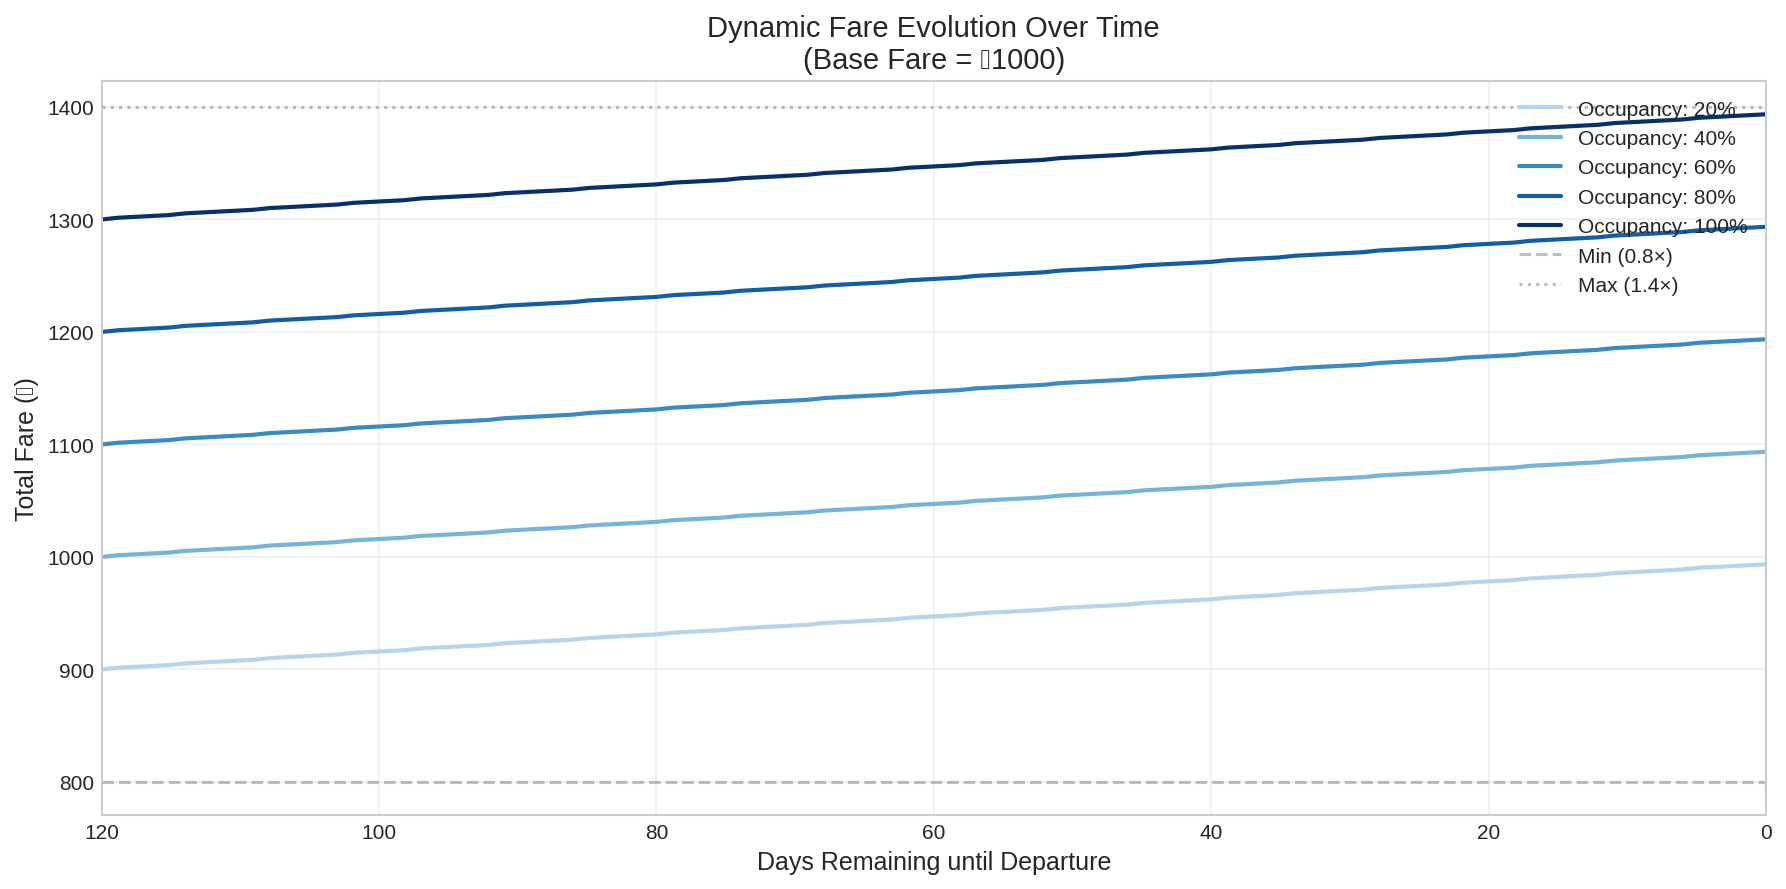
\includegraphics[width=\columnwidth]{fare_evolution.png}
    \caption{Dynamic fare evolution over the 120-day booking window
            for five seat occupancy levels (base fare Rs.\,1000).
            Dashed lines mark the 0.8$\times$ floor and 1.4$\times$
            ceiling. Fares rise as seats fill and as departure
            approaches; the two effects are additive.}
    \label{fig:evolution}
\end{figure}
% ---------------------------------------------------------------
 
%--------------------------------------------------------------------------------
\section{Results}
%--------------------------------------------------------------------------------
 
\subsection{Fare Multiplier Distribution}
 
Applying the model to all 84 Vande Bharat trains at their simulated average occupancies produces fare multipliers that cluster between 1.10$\times$ and 1.25$\times$ for Chair Car, with a mean around 1.21$\times$. Executive Chair multipliers are slightly lower on average (mean $\approx 1.17\times$) and more dispersed, which is expected given the 92\% EC-to-CC occupancy ratio built into the simulation. In both cases, no train hits the 1.4$\times$ cap under default parameters, leaving headroom for weekend and festival adjustments without breaching the guardrail.
 
% ---------------------------------------------------------------
% IMAGE SUGGESTION 3:
% Insert the fare multiplier distribution histograms here
% (vandebharat_fare_distribution.png).
% The two panels show the CC (blue) and EC (orange) distributions
% with the base fare (1.0x) and mean multiplier marked, making the
% results in this paragraph concrete.
% Suggested caption:
\begin{figure}[h!]
\centering
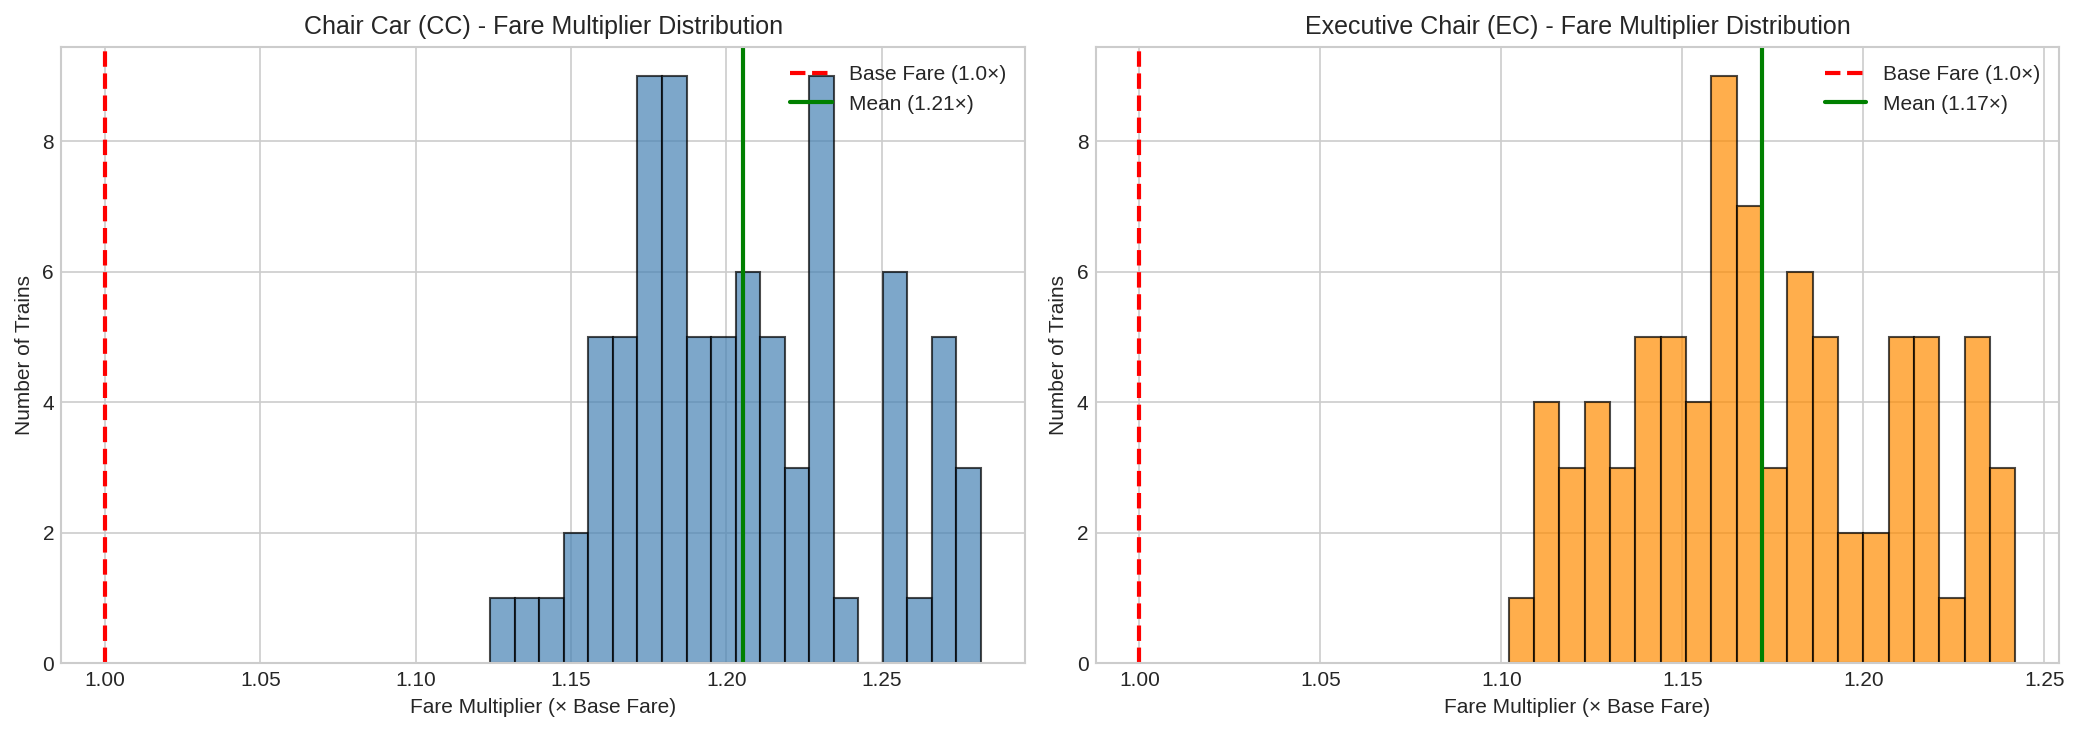
\includegraphics[width=\columnwidth]{vandebharat_fare_distribution.png}
\caption{Fare multiplier distributions across 84 Vande Bharat
            trains under the Singh et al.\ model ($w=0.187$, $M=0.5$).
            Left: Chair Car (mean 1.21$\times$). Right: Executive
            Chair (mean 1.17$\times$). No train reaches the 1.4$\times$
            cap under base parameters.}
\label{fig:dist}
\end{figure}
% ---------------------------------------------------------------
 
\subsection{Revenue Gains by Route}
 
Table~\ref{tab:revenue} summarises the combined revenue impact. Chair Car gains are larger in absolute rupee terms because of the much higher seat count (780 vs 104), while the EC gain per seat is comparable.

\begin{table}[h!]
\centering
\small
\caption{Revenue impact of dynamic pricing across 84 Vande Bharat trains (one run each, both directions averaged)}
\label{tab:revenue}
\begin{tabular}{lrrr}
\toprule
\textbf{Class} & \textbf{Current} & \textbf{Dynamic} & \textbf{Gain \%} \\
\midrule
Chair Car (CC)    & Rs. 1105 & Rs. 1332 & $\sim$21\% \\
Executive Chair (EC) & Rs. 2050 & Rs. 2398 & $\sim$17\% \\
\bottomrule
\end{tabular}
\end{table}

At the route level, Howrah$\to$Kamakhya stands out as the highest-gain train in both CC and EC --- unsurprisingly, as it is the sleeper variant with the highest occupancy simulation scores. Other consistently high-gain routes include Varanasi$\to$New Delhi (served by multiple pairs), H.\ Nizamuddin$\to$Khajuraho, and New Delhi$\to$Sri Mata Vaishno Devi Katra, all of which are medium-distance pilgrimage or tourism corridors with few viable competing transport options --- exactly the route profile Singh et al.\ recommend for dynamic pricing deployment.
 
% ---------------------------------------------------------------
% IMAGE SUGGESTION 4:
% Insert the revenue gain bar charts here (vandebharat_revenue_gain.png).
% The two panels rank the top 10 routes for CC (blue) and EC (orange)
% by revenue gain in lakhs, making the route-level discussion above
% visually concrete and easy to compare.
% Suggested caption:
\begin{figure}[h!]
\centering
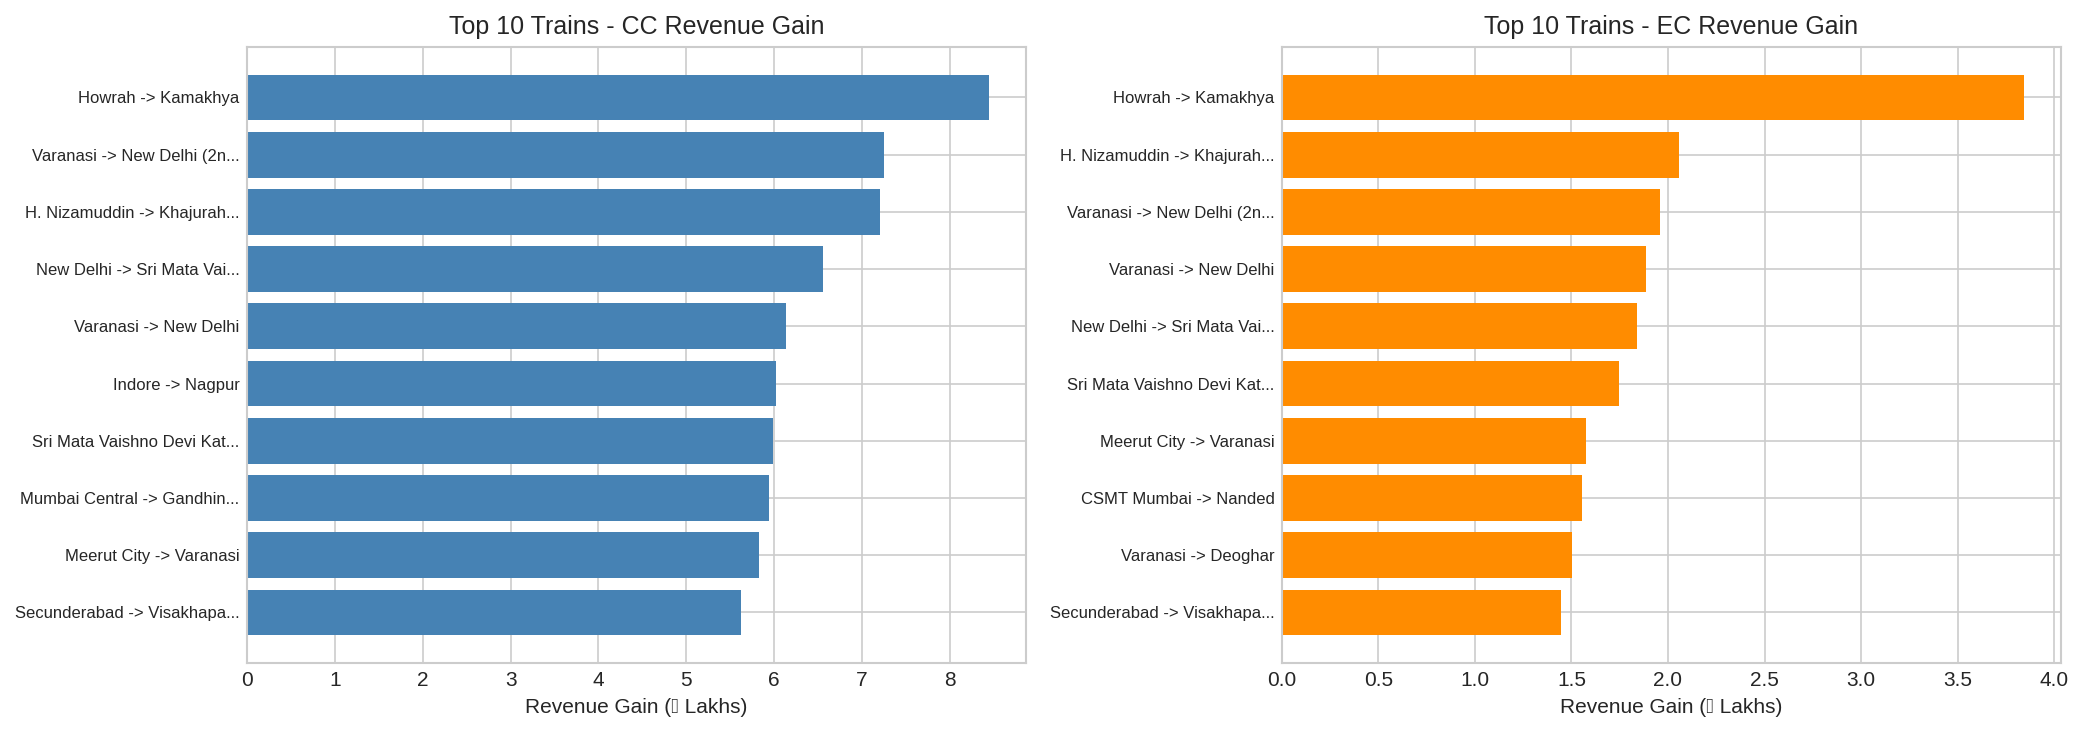
\includegraphics[width=\columnwidth]{vandebharat_revenue_gain.png}
\caption{Top 10 Vande Bharat routes by estimated revenue gain under
            dynamic pricing. Left: Chair Car. Right: Executive Chair.
            Howrah--Kamakhya dominates in both classes; tourist and
            pilgrimage corridors feature prominently throughout.}
\label{fig:gain}
\end{figure}
% ---------------------------------------------------------------

%--------------------------------------------------------------------------------
\section{Extra Variables and Future Proposal}
%--------------------------------------------------------------------------------

\subsection{Additional Pricing Factors}
 
The base model can be extended in three straightforward ways that the paper explicitly sanctions. A \textit{weekend adjustment} of $+25\%$ on the multiplier covers Saturday and Sunday departures, where leisure demand is concentrated and price sensitivity is lower. A \textit{festival-week adjustment} of the same magnitude handles high-demand periods around Diwali, Holi, Navratri, and the summer school holiday window. An \textit{overnight adjustment} applies to trains running between 10\,pm and 6\,am, which typically attract business travellers willing to pay a premium for the convenience of sleeping on board. These three flags are additive and can combine up to a multiplier of $M = 0.5 \times 1.25^3 \approx 0.977$, which in practice pushes fares toward but not past the 1.4$\times$ cap on high-occupancy runs.
 
\subsection{What the Model Does Not Capture}
 
A few important limitations deserve honest acknowledgement. The weight parameter $w$ is derived from historical booking patterns and is constant over the 120-day window, whereas actual demand elasticity likely varies by season and by how far in advance the analysis is being done. The model also has no competitor-fare feedback loop: Singh et al.\ flag the risk that fares approaching airline levels on premium corridors can push travellers to fly, but the current implementation has no mechanism to detect or respond to this. Finally, the occupancy data here is simulated, not observed. The directional rankings are likely stable, but any specific rupee figure should be treated with appropriate caution until validated against real IRCTC booking data.
 
\subsection{Directions for Further Work}
 
The most impactful near-term extension would be to replace the simulated occupancy with actual IRCTC booking curves, which would also allow the weight parameter to be recalibrated route by route rather than fixed at the paper's six-train average. Beyond that, a forecasting layer --- whether a simple time-series model or an LSTM trained on historical bookings --- would transform this from a snapshot analysis into a forward-looking pricing engine. Incorporating competitor fare data from airline aggregators would address the price-ceiling concern. A seasonal analysis covering at least one full year is needed before any recommendation could responsibly be taken to an operational setting.

\begin{thebibliography}{99}
 
\bibitem{singh2023}
Singh, K., Dhake, P., \& Narayanaswami, S. (2023).
A dynamic pricing strategy model for Indian Railways.
\textit{Journal of Revenue and Pricing Management}, 23, 295--304.
 
\bibitem{mint2017}
Mint (2017). Flexi-fare scheme: Railways earns additional Rs.\,540 crore in 11 months.
\textit{Livemint}.
 
\bibitem{data}
Vande Bharat Complete Dataset (2026).
\url{https://drive.google.com/drive/folders/1GWaHyWj9oSI-mY28Z6yLyC2wwyIXtaG6}
 
\end{thebibliography}
 
\end{document}